\chapter{Context}
\markboth{Context}{Context}
\label{chapIntroduction}
%\minitoc

\marginnote{\textsl{Machine learning}}[1cm]
In the past decade due to the boom in Information Technology (IT) companies, more investment has gone into developing both computational infrastructure and methods. One of the ubiquitous methods developed due to this investment is that of Machine Learning. Learning algorithms look for patterns in data to learn from them and make decisions. They are used in web search, optimization, spam filtering, ad placement, stock trading, healthcare, manufacturing, space exploration, particle physics, security, and lot more. The speed and adaptability of learning methods are changing everything around us one algorithm at a time \cite{domingos2015master}. The World Economic Forum, Davos 2016 \cite{schwab2016fourth} has dubbed this as the fourth industrial revolution; first was steam powered, second was electrically powered, third was IT powered, fourth will be powered by artificial intelligence algorithms.

\marginnote{\textsl{Aircraft design}}[1cm]
In comparison aircraft design is almost a century old field, the first successful flight being by the Wright brothers in 1903 \cite{wright1934we}. Currently, the design of an aircraft is a highly-iterative optimization process. Based on the initial target objectives and general trends, aircraft designers define the objectives for domain specific departments (eg. aerodynamics design or structural design). These objectives further trickle down to more dedicated teams and tasks (eg airfoil design or fuselage design). This gives rise to a huge Multi-Disciplinary Optimization (MDO) problem. Teams come up with individual constraints, they iterate around their domains, interact with neighboring domains and negotiate overlapping constraints. Teams negotiate and solidify individual objectives and constraints to find the optimized design for an aircraft. An optimized design as close to the initial target objectives, an optimized design taking into account the sparse infrastructure, human and economic limitations. This is a massive MDO problem spanning almost a decade, costing billions and involving thousands of people. 

\begin{figure}[!ht]
\label{figPhasesOfAircraftDesign}
  \centering
  
    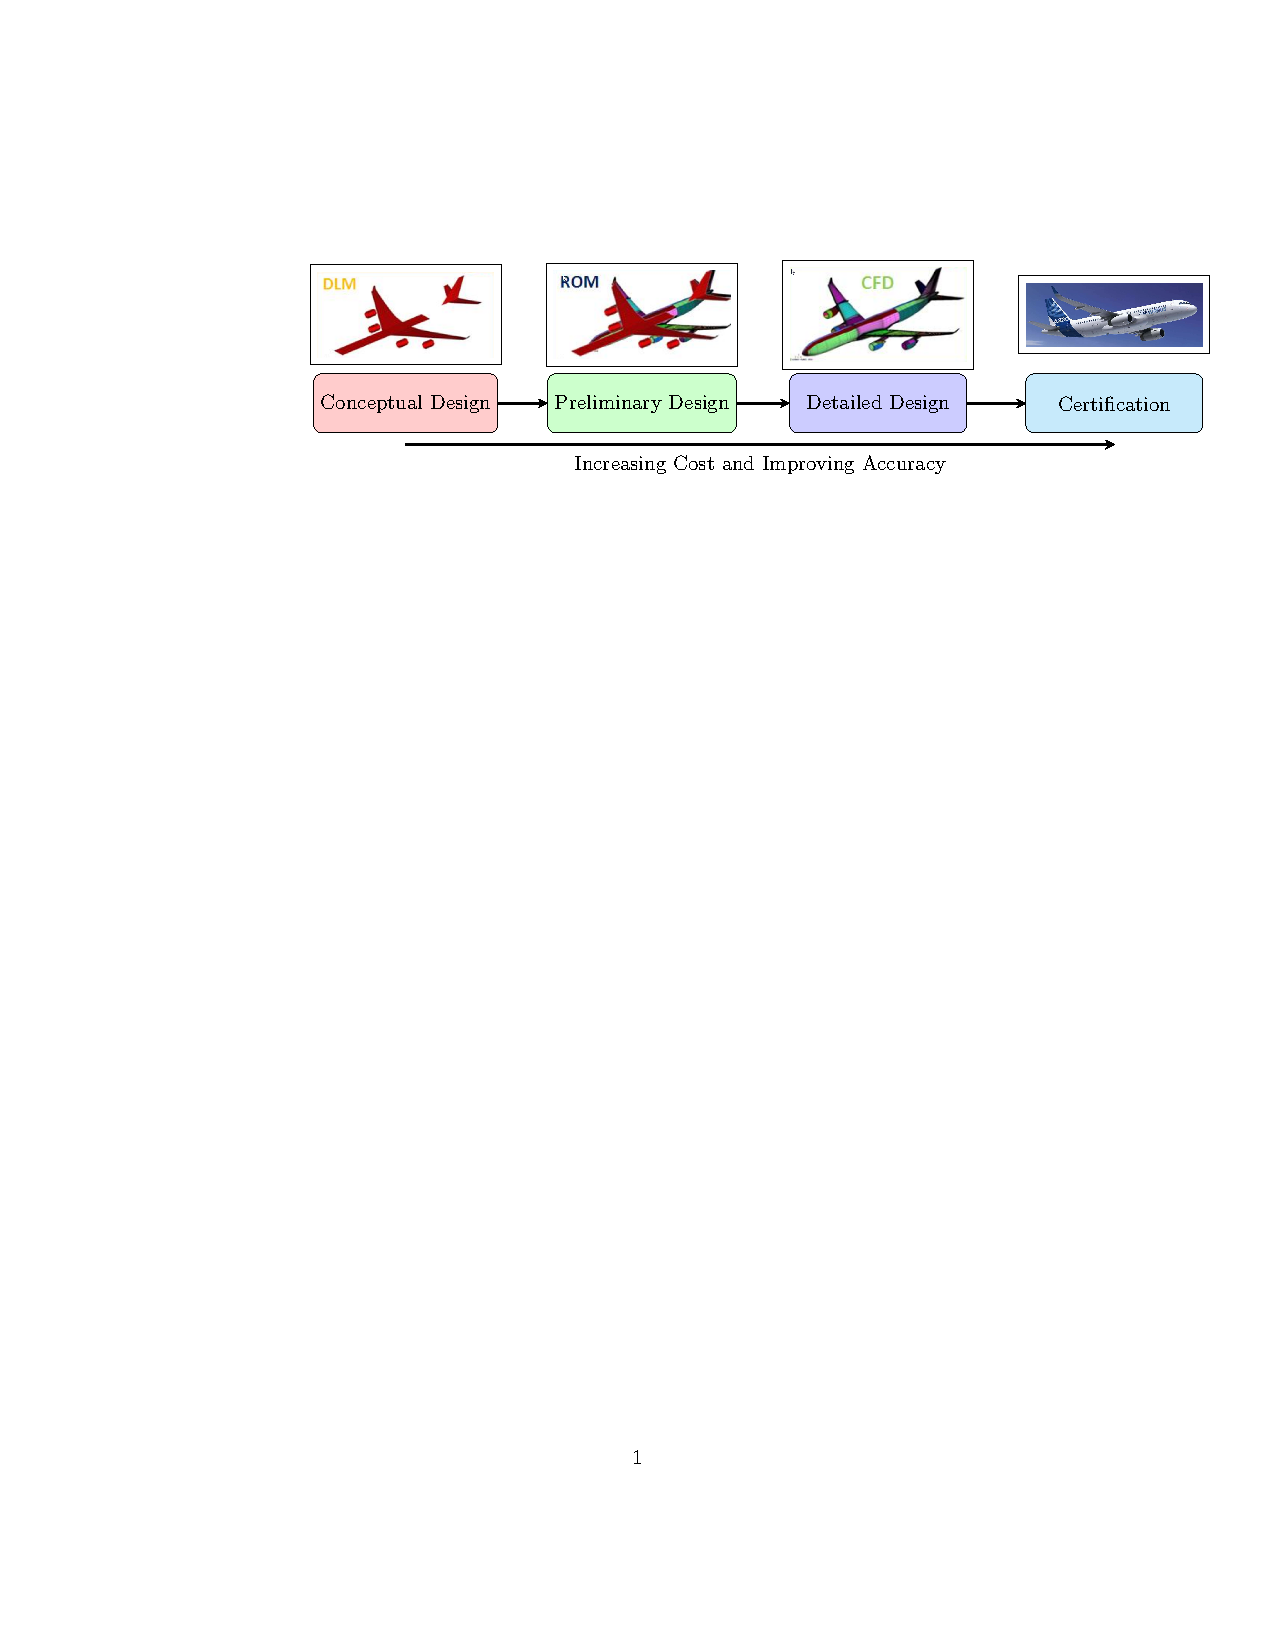
\includegraphics[clip, trim=4.5cm 19cm 0.5cm 4cm,width=0.95\textwidth]
    {images/part1/aircraftDesignCycleFlowChart}
  
  \caption{Phases of an aircraft design cycle}
\end{figure}

\section{Aircraft design cycle}\label{secSircraftDesignCycle}
\marginnote{\textsl{Design phases}}[1cm]
To simplify this process an aircraft design is broken down into several design phases (figure \ref{figPhasesOfAircraftDesign}). Each phase requires an ever increasing amount of predictions and fidelity. Preliminary design phase requires a few low-fidelity design trade-offs between major disciplines. Whereas, during detailed design phase, intensive intra-disciplinary and inter-disciplinary optimization's take place. Finally, during the flight-test and certification phase capability to predict real-time can provide significant gains in reducing the flight-test phase. These analyses cover large parts of flight envelope and require high-fidelity predictions. Hence the capability to accurately and quickly predict is an integral part of an aircraft design cycle \cite{raymer2012aircraft}. 

\marginnote{\textsl{Need for Speed}}[1cm]
In the last decade high-fidelity, physics based, mathematical simulations have become central to designing an aircraft. However, high-fidelity simulations are computationally expensive, this is the case for several Computational Fluid Dynamics (CFD) and Finite Element Method (FEM) based solvers. Due to this high cost high-fidelity simulations are launched only for a few carefully chosen design configurations. This results in inefficient exploration of the the design space and thus a non-optimal design. A common strategy to speed up simulations is by reducing the physical complexity of the model to make quick predictions. As an example linear potential flows (simpler aerodynamic model), or coarser FEM meshes (simpler structural model) are regularly used during the preliminary design phase \cite{cummings2015applied}. While this is an acceptable practice during the preliminary design phase, during the detailed design phase physical complexity is needed to find a robust optimum design point \cite{raymer2012aircraft}.

\marginnote{\textsl{Need for accuracy}}[1cm]
Instead of approximating physical complexity, surrogate models\footnote{Surrogate models, learning algorithms and machine learning models will be used interchangeably throughout this manuscript} simplify mathematical complexity \cite{verveld2016reduced}. Surrogate models learn patterns between the input and output dataset and then are used to make predictions on the desired point. This property is very useful in quickly exploring the design space and finding a robust design point \cite{forrester2008engineering}. Moreover, surrogate models are commonly passed across disciplines to perform inter-disciplinary optimizations. For example, a loads department would prefer running a quick surrogate model over the costly CFD model while performing the load's loop \cite{bartoliAIAA2017, bartoliAGILE2017}.  

\marginnote{\textsl{Deduction vs Induction}}[1cm]
The main difference between the engineering design and surrogate modeling can be explained by the difference between deduction and induction \cite{domingos2012few} (figure \ref{fig:engineeringDesignVsSurrogateModelling}). Engineering design is deduction: where a very general formula is applied to a particular case (figure \ref{figDeduction}). The basics of Newtonian physics, when applied to a particular aircraft geometry, give inertial loads. The basics of aerodynamics, when applied to a particular set of aircraft geometry and aircraft states, give out aerodynamic pressures. Engineering design takes global rules and applies them to local configurations. Whereas, surrogate modeling is induction: it looks at local features and data, tries to find similarity measures between them and gives a global formula for the process (figure \ref{figInduction}). For example, an algorithm to detect faces in images will look at several images with and without faces, learn a facial pattern and make predictions on new images \cite{marszalek2007semantic}. We here see a possible complementary relationship between engineering design and machine learning; where engineering design needs models to generate data, machine learning needs data to generate models.

\begin{figure}[!ht]\label{fig:engineeringDesignVsSurrogateModelling}
  \centering
  \subfigure[Engineering design - Deduction: The figure shows an application of a general rule to a particular case.]
  {
    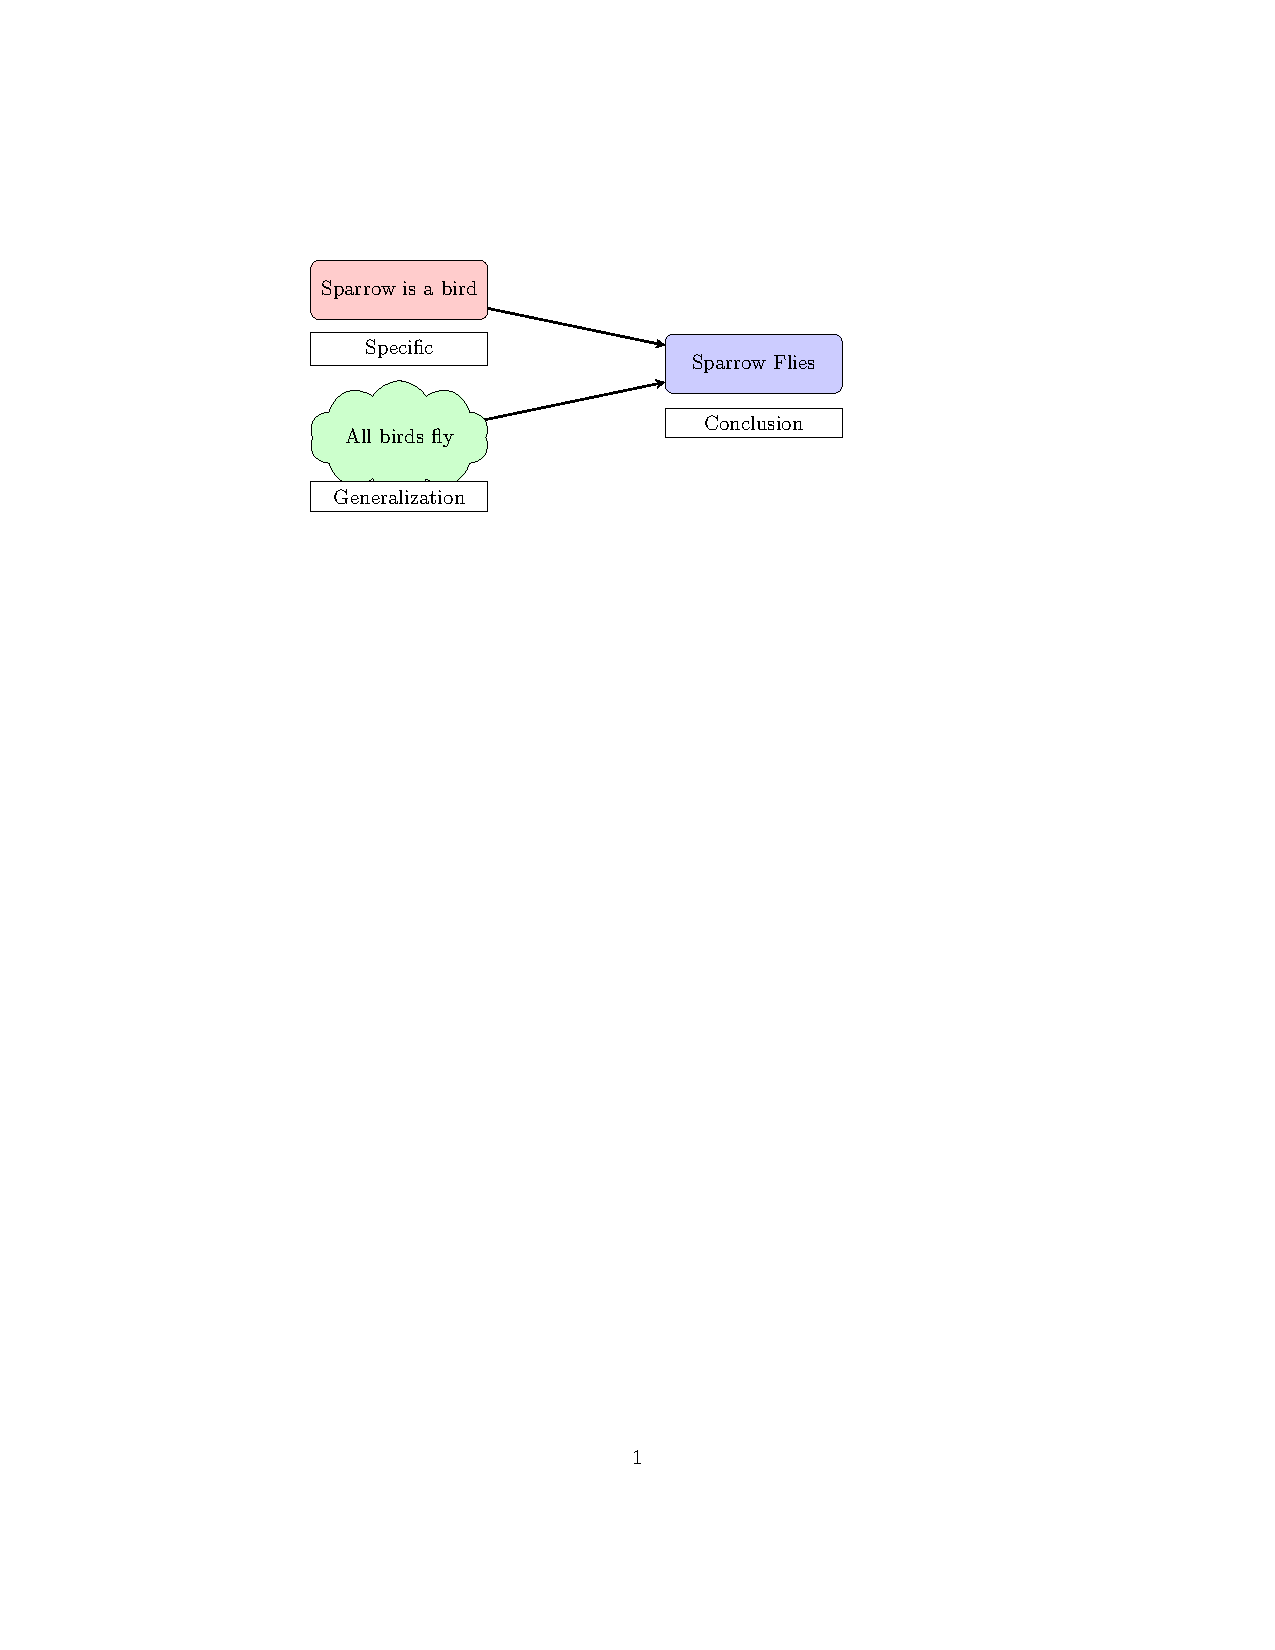
\includegraphics[clip, trim=4.5cm 19cm 4.5cm 4cm,width=0.45\textwidth]
    {images/part1/deduction}
    \label{figDeduction}
  }\quad
  \subfigure[Surrogate modelling - Induction: The figure shows how multiple examples can be used to infer underlying rules or patterns that govern the system.]
  {
    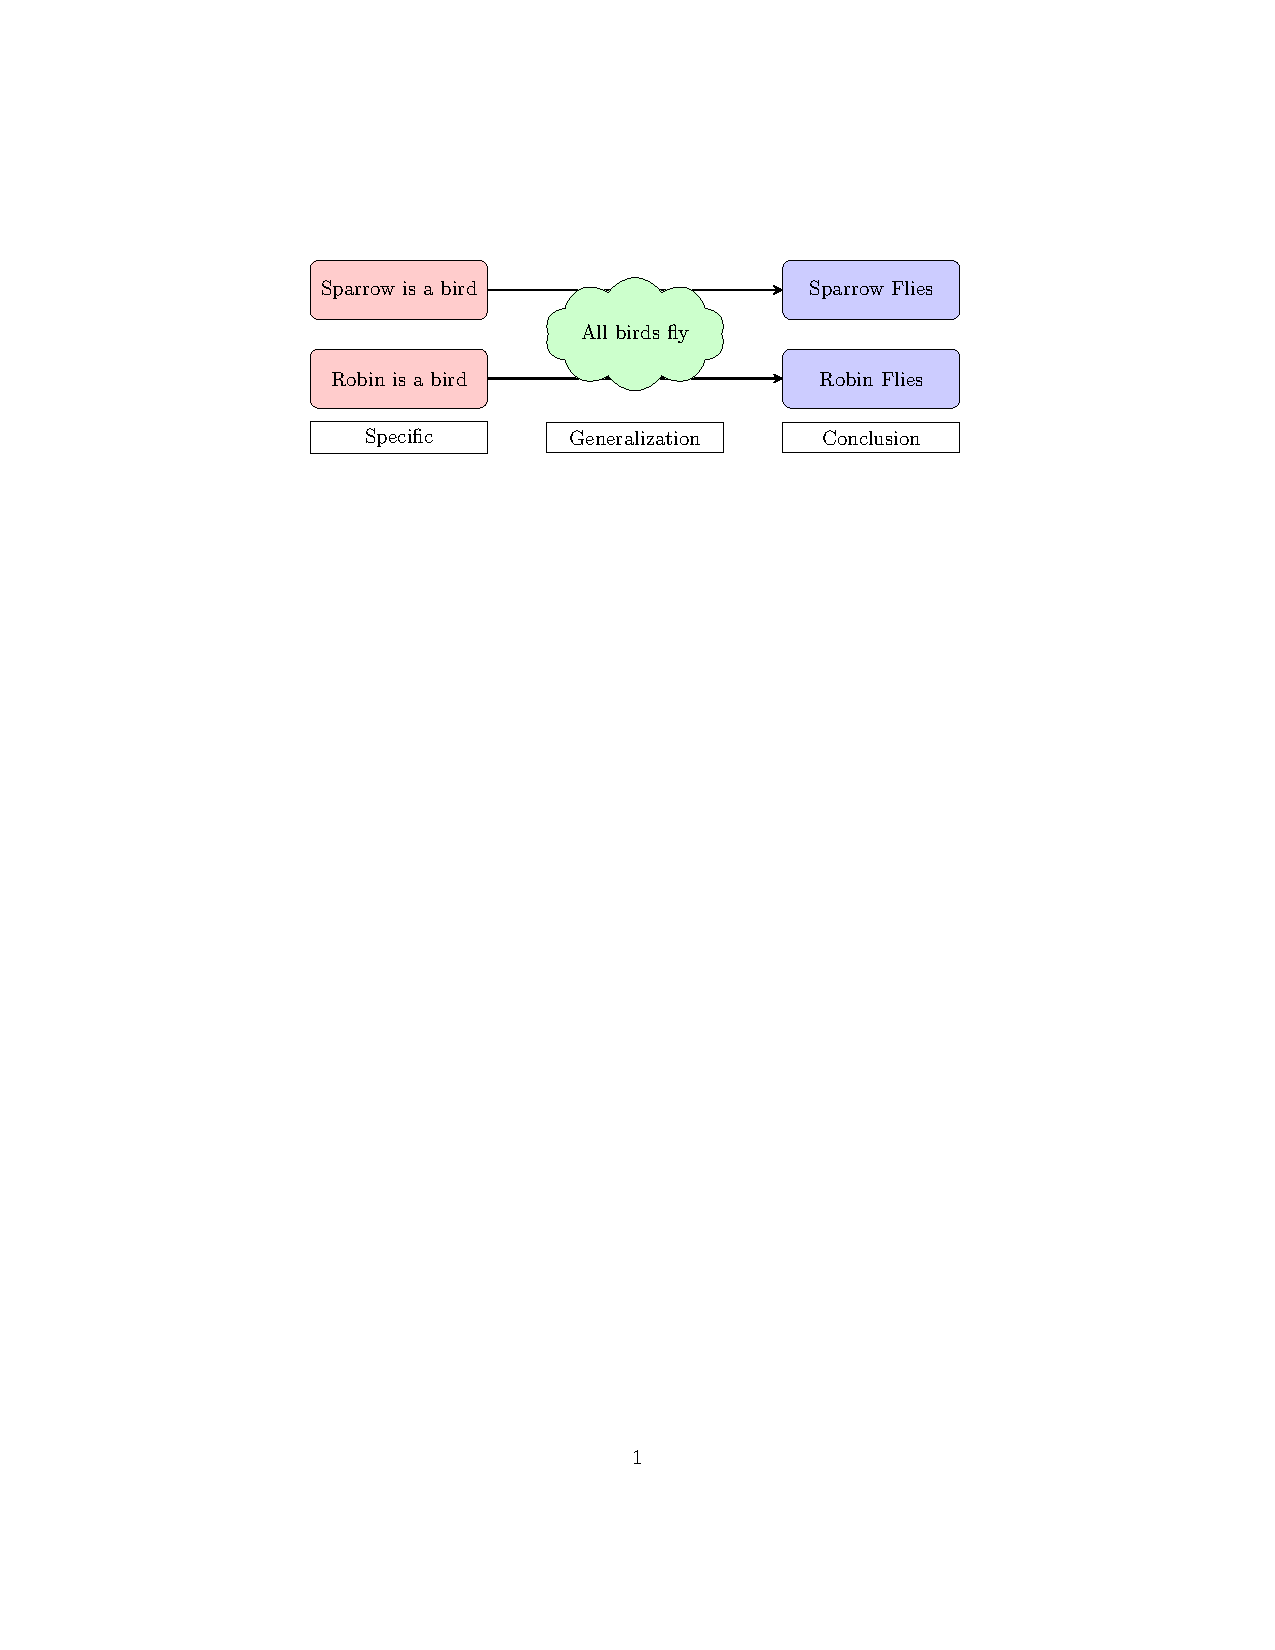
\includegraphics[clip, trim=4.5cm 20cm 4.5cm 4cm,width=0.45\textwidth]
    {images/part1/induction}
    \label{figInduction}
  }\quad
  \caption{Induction vs Deduction}
\end{figure}

\marginnote{\textsl{Developing faster models}}[1cm]
Since models are an integral part of any engineering design, model building in aircraft engineering was traditionally outsourced to research institutes. Researchers perform iterative experiments in a controlled environment and discover patterns between the physics of the system. For example, it took 200 years to iteratively develop the Gas law \footnote{$Pressure \times Volume \propto numberOfMoles \times Temperature$}, Boyle's law in 1600's found the relation between Pressure and Volume, Charle's Law in 1787 discovered the relationship between Volume and Temperature, while Gay-Lussac's Law in 1809 discovered the relationship between Pressure and Temperature \cite{clapeyron1834memoire}. This is a rigorous and time-consuming method of developing models. Machine learning is a much more elegant method of building models. Using data and few basic assumptions, automatic models can be built between desired inputs and outputs. For example, while the first model of a neural network was proposed in 1950's \cite{kleene1951representation}, neural networks are today used daily for tasks such as tagging cat photos on facebook and converting speech to text\footnote{I wrote a fourth of this thesis using a text to speech software}. In this thesis, we wish to automatically build models for aircraft design tasks primarily to be used during the detailed design phase and certification phase. 


\section{Machine Learning}\label{secMachineLearning}
\marginnote{\textsl{Components of learning}}[1cm]
The core objective of learning algorithms is to find a transformation function between the inputs and outputs. There are three main components in a learning algorithm:
\begin{enumerate}
\item \textbf{Representation}: A learning algorithm starts with a family of functions. For example, a linear model is a family of linear functions, a trigonometric model defines a family of trigonometric functions. If an algorithm is not able to represent the actual function in its family of functions, it will find the closest function in its hypothesis space\footnote{The term family of functions, hypothesis space and representation will be used interchangeably throughout this manuscript}.
\item \textbf{Evaluation}: Some measure is needed to distinguish a good function from a bad function in the chosen hypothesis space. This measure is termed as evaluation; one example is the least squares error commonly used in many learning algorithms. 
\item \textbf{Optimization}: Finally, the algorithm iteratively searches in its hypothesis space to find the best possible function explaining the data. The choice of optimizer defines the speed of learning and is also important if there are multiple minima in the evaluation criteria.
\end{enumerate}

\marginnote{\textsl{Bias vs Variance}}[1cm]
Surrogate models suffer from the bias vs variance trade-off (figure \ref{figBiasVsVariance}), formalized by `Wolpert' in his famous "no free lunch theorem" \cite{wolpert1997no}. The constituent functions in a hypothesis space represent the bias or assumptions of the learning algorithm (eg. linear functions for linear regression). In the absence of sufficient assumptions, the family of functions in the search space becomes very large which leads to high variance or over-fitting in the surrogate model (figure \ref{subFigpredictionPoly15}). On the contrary, wrong bias means that the true transformation function ($f$) does not exist in the hypothesis space. In this case, the learning algorithm finds the function closest to $f$ in its hypothesis space and leads to under-fitting (figure \ref{subFigpredictionPoly6}).

\begin{figure}[!ht]
  \centering
    \subfigure[{High-bias and low variance}]
  {
        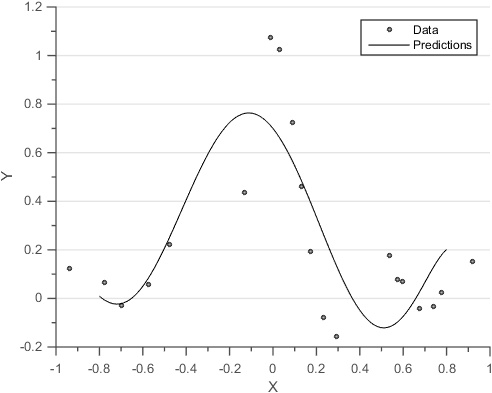
\includegraphics[width=0.29\textwidth]
        {images/part1/predictionPoly6}
        \label{subFigpredictionPoly6}
  }\quad
\subfigure[{Low bias and High variance}]
  {
        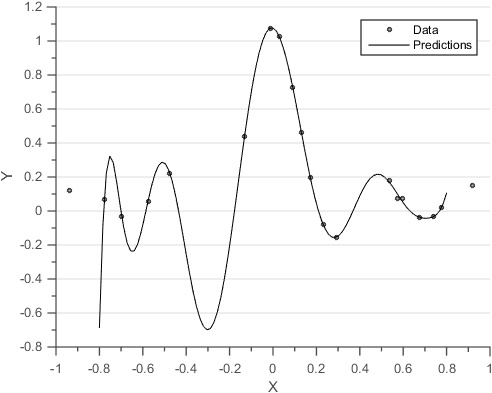
\includegraphics[width=0.29\textwidth]
        {images/part1/predictionPoly15}
        \label{subFigpredictionPoly15}
  }\quad
  \subfigure[{Bias replaced with lots of data}]
  {
        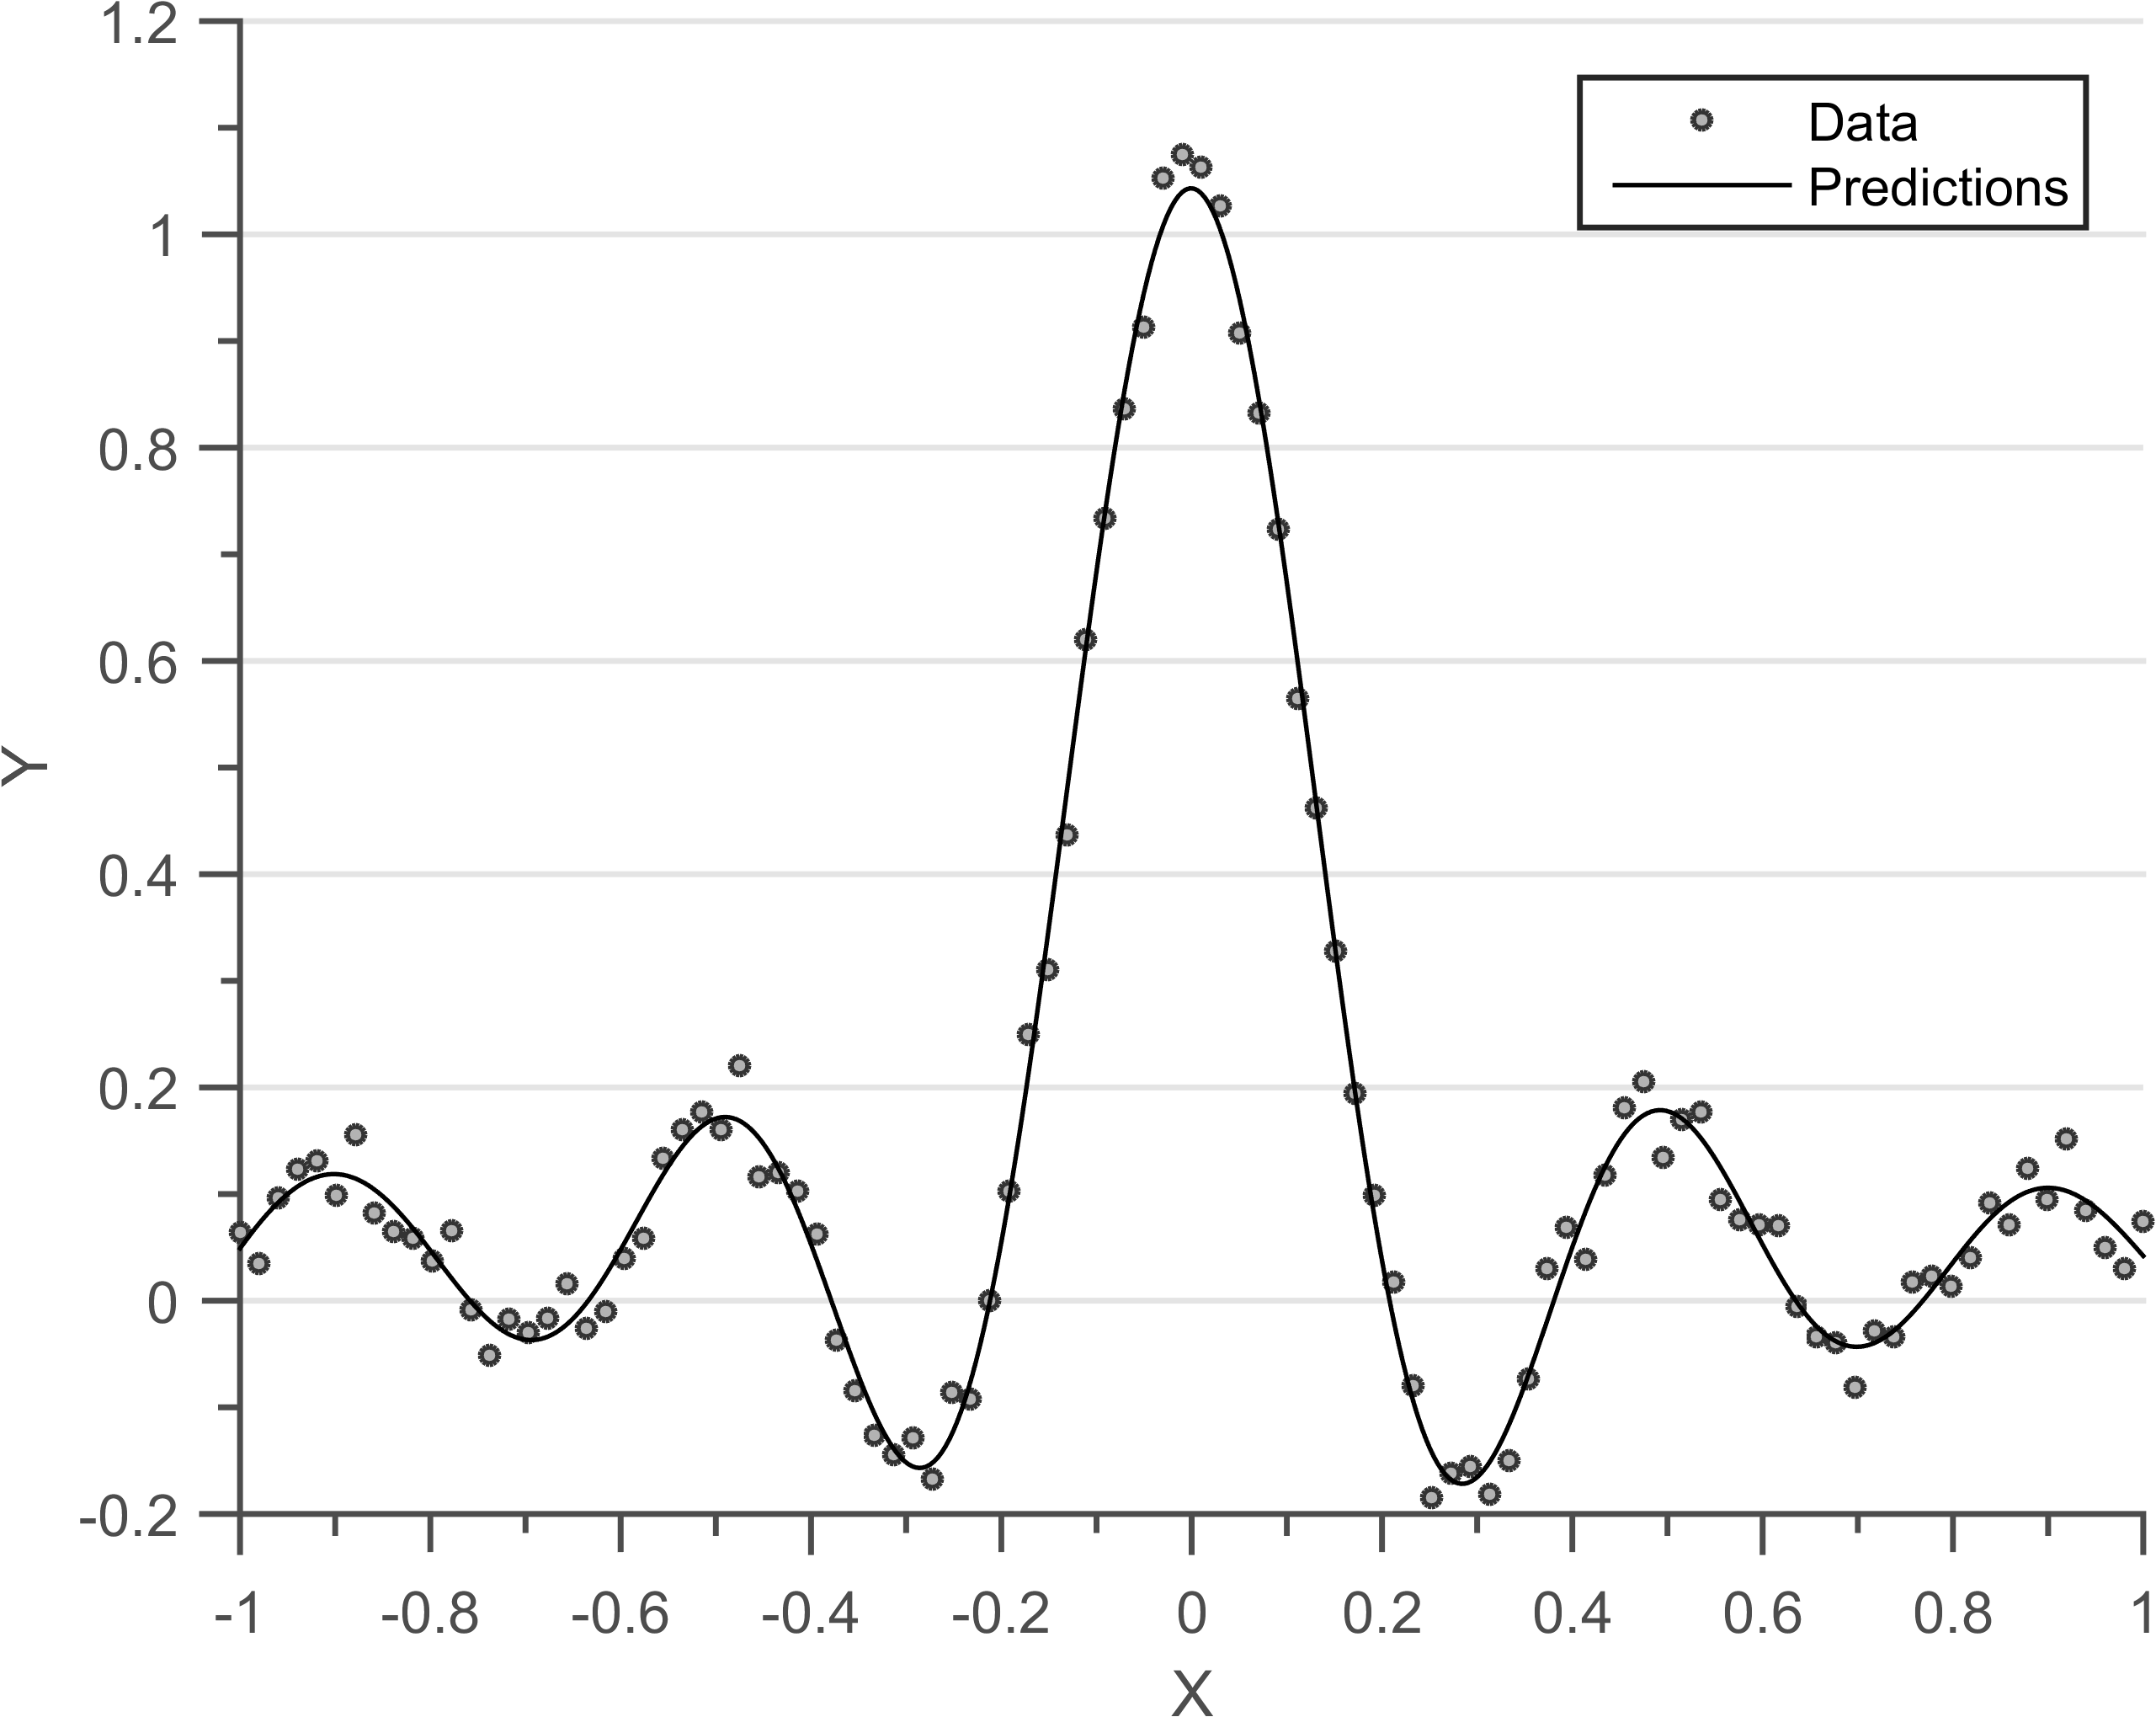
\includegraphics[width=0.29\textwidth]
        {images/part1/posteriorSEInitialAtI100}
        \label{subFigposteriorSEInitialAtI100}
  }\quad
       \caption{Bias vs Variance trade-off}
       \label{figBiasVsVariance}
\end{figure}



\marginnote{\textsl{Soft and hard constraints}}[1cm]
One method to overcome this trade-off is by using lots and lots of data. Data acts as a hard constraint for learning algorithm, imagine a family of all possible continuous 2-dimensional functions in the range of $x \in [-1, 1]$ and $y \in [-1, 1]$. What will happen, given an observation $(x = 0, y = 0)$. All the functions that do not pass through this point will be eliminated, the new data point has basically reduced the possible family of functions. Whereas, bias acts as soft constraint, we can use the bias of linearity or smoothness to reduce our hypothesis space. Therefore, both bias and data help in reducing the hypothesis space\footnote{Bias can also be looked upon as distilled knowledge or patterns gained after interpreting huge amounts data}. Given access to more and more data, we can progressively reduce the bias in learning models thereby relying more on true evidence. This is also the main concept behind deep learning, where several layers of neural networks define a very large hypothesis space \cite{Goodfellow-et-al-2016, lecun2015deep}. 

Unfortunately in aircraft design, generating a huge amount of accurate data is a costly exercise, for example a high fidelity CFD simulation runs for weeks \cite{murthy2014computational, jameson2012computational, forrester2008engineering} and a flight-test campaign costs millions of euros \cite{fox2004test}. On another hand due to centuries of research and tinkering, we have a treasure trove of prior information about the physical systems. We propose to build better machine learning models by integrating the time-tested prior knowledge of physical systems with experimental data. 

\begin{mdframed}[hidealllines=true,backgroundcolor=blue!20]
\marginnote{\textsl{Contribution}}[1cm]
The main contribution of this thesis is to provide a framework on how to combine the prior knowledge from a physical system and add it to a learning algorithm. A model generated from merging of the two methodologies will be both consistent with the physics of the system and be quicker to evaluate. We integrate three types of prior knowledge by answering the following questions:
\begin{enumerate}
\item \textbf{Pattern}: How to add \textit{apriori} information of a pattern in a learning algorithm? For example, given that shock is a discontinuous change in pressure, how to predict the position of shock on an airfoil (part \ref{partIncorporatePattern}). 
\item \textbf{Relationships}: How to add \textit{apriori} information of relationships between measurements? For example given $Loads = \int Pressures$, how to make a robust loads model when we measure both pressures and loads (chapter \ref{chapAddingEquationsInGP}).
\item \textbf{Simulation model}: How to merge \textit{apriori} information of simulations with experiments? For example, given a simulation model and experimental data how to perform extrapolations on experimental data(chapter \ref{chapMultiTaskExtrapolation}). 
\end{enumerate}

To integrate the prior information we propose to use a Bayesian inference for model building. Bayesian inference is a method of statistical inference in which Bayes theorem is used to update an initial probability (prior) as more and more evidence becomes available the final probability (posterior) gives our estimate. More specifically, we will use the Gaussian Processes (GP) Regression framework which is a subset of the Bayesian Inference algorithms to define prior information of physical systems. But, before deep diving into the details of GP let us have a look at a simple Bayesian Linear Regression algorithm.
\end{mdframed}

\section{Bayesian Linear Regression}\label{secBayesianModelling}
\sloppy Suppose we have access to a training set of observations (or outputs) $Y = (y(x_{1}); \ldots ; y(x_{i}); \ldots ; y(x_{N}))$, evaluated at a set of known inputs $X = (x_{1}; \ldots ; x_{i}; \ldots; x_{N})$, and we wish to predict $y(x_{*})$ at a test input $x_{*}$. The input and output can be multi-dimensional; $x_{i} \in \mathbb{R}^{D_{inputs}}$ and $y(x_{i}) \in \mathbb{R}^{D_{outputs}}$. The process of learning the transformation function $f$ to make prediction at a new point is called as regression. In the following section we follow formulation for Bayesian Linear Regression provided by \cite{mackay2003information}.

\marginnote{\textsl{Basis functions}}[1cm]
A simple method to perform regression is by assuming a form of the function $f$, then minimizing the error between the true measurements and assumed form to estimate the parameters of $f$. The function is written in terms of basis functions $\phi(x)$. For example when $\phi(x) = \{1, x\}^{T}$ we are performing linear regression, when $\phi(x) = \{1, x, x^{2}, \ldots, x^{L}\}^{T}$ we are performing $L^{th}$ order polynomial regression. We will focus on linear regression in this section and hence $\phi(x) = \{1, x\}^{T}$.

\begin{equation}\label{eqBayesianLinearRegression}
f(x_{i}) = \begin{Bmatrix}
1 & x
\end{Bmatrix}  \begin{Bmatrix}
w_{0}\\ 
w_{1}
\end{Bmatrix}
\quad \quad y(x_{i}) = f(x_{i}) + \epsilon
\end{equation}

\marginnote{\textsl{Likelihood}}[1cm]
Here, $w$ are the parameters of the function, such that $w_{0}$ denotes the intercept and $w_{1}$ denotes the slope of the regression model. The measurements are corrupted by independent white noise $\epsilon$, such that the noise is a random variable sampled from a white noise Gaussian\footnote{$\Pr[\epsilon] = \mathcal{N}(0, \sigma_{n}) = \frac{1}{\sqrt{2\pi\sigma_{n}^{2}}}\exp^{-\frac{\epsilon^{2}}{2\sigma_{n}^{2}}}
$} with variance $\sigma_{n}^{2}$. The above equations \ref{eqBayesianLinearRegression} can be combined to result in the likelihood $\Pr[Y\mid X, w]$

\begin{equation}\label{eqBayesianLikelihood}
\begin{aligned}
\Pr[Y \mid X, w]  & = \prod \Pr[y_{i}\mid x_{i}, w]\\
                & = \prod \mathcal{N}[[1, x_{i}]w , \sigma_{n}^{2}]\\
                & = \mathcal{N}(X^{T} w, \sigma_{n}^{2}I_N)    
\end{aligned}
\end{equation}

The notation $\Pr[Y \mid X, w]$ symbolizes probability distribution of observations $Y$ at the inputs $X$ given the parameter $w$. The notation $\mathcal{N}[\mu , \Sigma]$ symbolizes a multi-variate Gaussian distribution for mean vector $\mu$ and covariance matrix $\Sigma$. $I_N$ is an identity matrix of size $N \times N$.

\marginnote{\textsl{Prior}}[1cm]
While performing Bayesian inference we specify a prior distribution to encode our assumptions on the parameters before we look at the observations. For this case, we put a zero mean Gaussian prior on our weights.

\begin{equation}\label{eqBayesianPrior}
\Pr[w] = \mathcal{N}(0, \Sigma_{Prior})
\end{equation}

The prior distribution on $w$ induces a prior distribution over functions parametrized by $w$, effectively we are defining family of functions $(\Pr[f(x_{i})] = \mathcal{N}(0, x_{i}^{T}\Sigma_{Prior}x_{i}))$ by placing a prior distribution over $w$. Once we have a prior distribution encoding our beliefs, we use Bayes rule to look at the observations and get a posterior distribution of parameters.

\begin{equation*}
posterior = \frac{likelihood \times prior}{marginal \quad likelihood}
\end{equation*}
\begin{equation}\label{eqBayesRule}
\Pr[w \mid Y, X] = \frac{\Pr[Y \mid X, w] \times \Pr[w]}{\Pr[Y \mid X]}
\end{equation}

\marginnote{\textsl{Marginal Likelihood}}[1cm]
The \textsl{marginal likelihood} is a normalization constant, for more details please refer to section \ref{secHyperParameter}. After, using the equation \ref{eqBayesianLikelihood}, \ref{eqBayesianPrior} and \ref{eqBayesRule} we can get the posterior distribution of weights as:

\begin{equation}\label{eqBayesianPosterior}
\Pr[w \mid Y, X]  = \mathcal{N}\left ( \frac{1}{\sigma_{n}^{2}} A^{-1}X Y , A^{-1} \right )
\end{equation}

Here, $A = \sigma_{n}^{-2}XX^{T} + \Sigma_{Prior}^{-2}$. Thus the posterior distribution for function $f$ at test point $x_{*}$ becomes:

\begin{equation}\label{eqBayesianFunctionalPosterior}
\Pr[f \mid x_{*}, X, y]  = \mathcal{N}\left ( \frac{1}{\sigma_{n}^{2}} x_{*}A^{-1}XY , x_{*}^{T}A^{-1}x_{*} \right )
\end{equation}

\marginnote{\textsl{Posterior}}[1cm]
The mean $\frac{1}{\sigma_{n}^{2}} x_{*}A^{-1}XY$ can be used as a prediction at the test point $x_{*}$, while the variance is a measure of uncertainty for this prediction. We can thus obtain the prediction $f(x_{*})$, using a prior set of beliefs (equation \ref{eqBayesianPrior}) and updating those beliefs using observations. 

\begin{mdframed}[hidealllines=true,backgroundcolor=lightgray!20]
\marginnote{\textsl{Experiment}}[1cm]
Suppose we have a toy dataset $\mathcal{D}_{1} = \{X = [-0.5, 0.33, 0.66], Y = [0, 0.5, 0.5]\}$ and want to find a function that fits this dataset using Bayesian Linear Regression. If we assume a prior distribution of parameter $w$ as defined by equation \ref{eqExperimentalPrior}, then the probability density of $w$ will look like figure \ref{subFigpriorBLR}.

\begin{equation}\label{eqExperimentalPrior}
\Pr \left [\begin{pmatrix}
w_{0}\\ 
w_{1}
\end{pmatrix} \right ] = \mathcal{N}\left [ \begin{pmatrix}
0\\ 
0
\end{pmatrix}, \Sigma_{P} = \begin{bmatrix}
1 & 0\\ 
0 & 1
\end{bmatrix} \right ]
\end{equation}
\end{mdframed}

\begin{figure}[!ht]
  \centering
            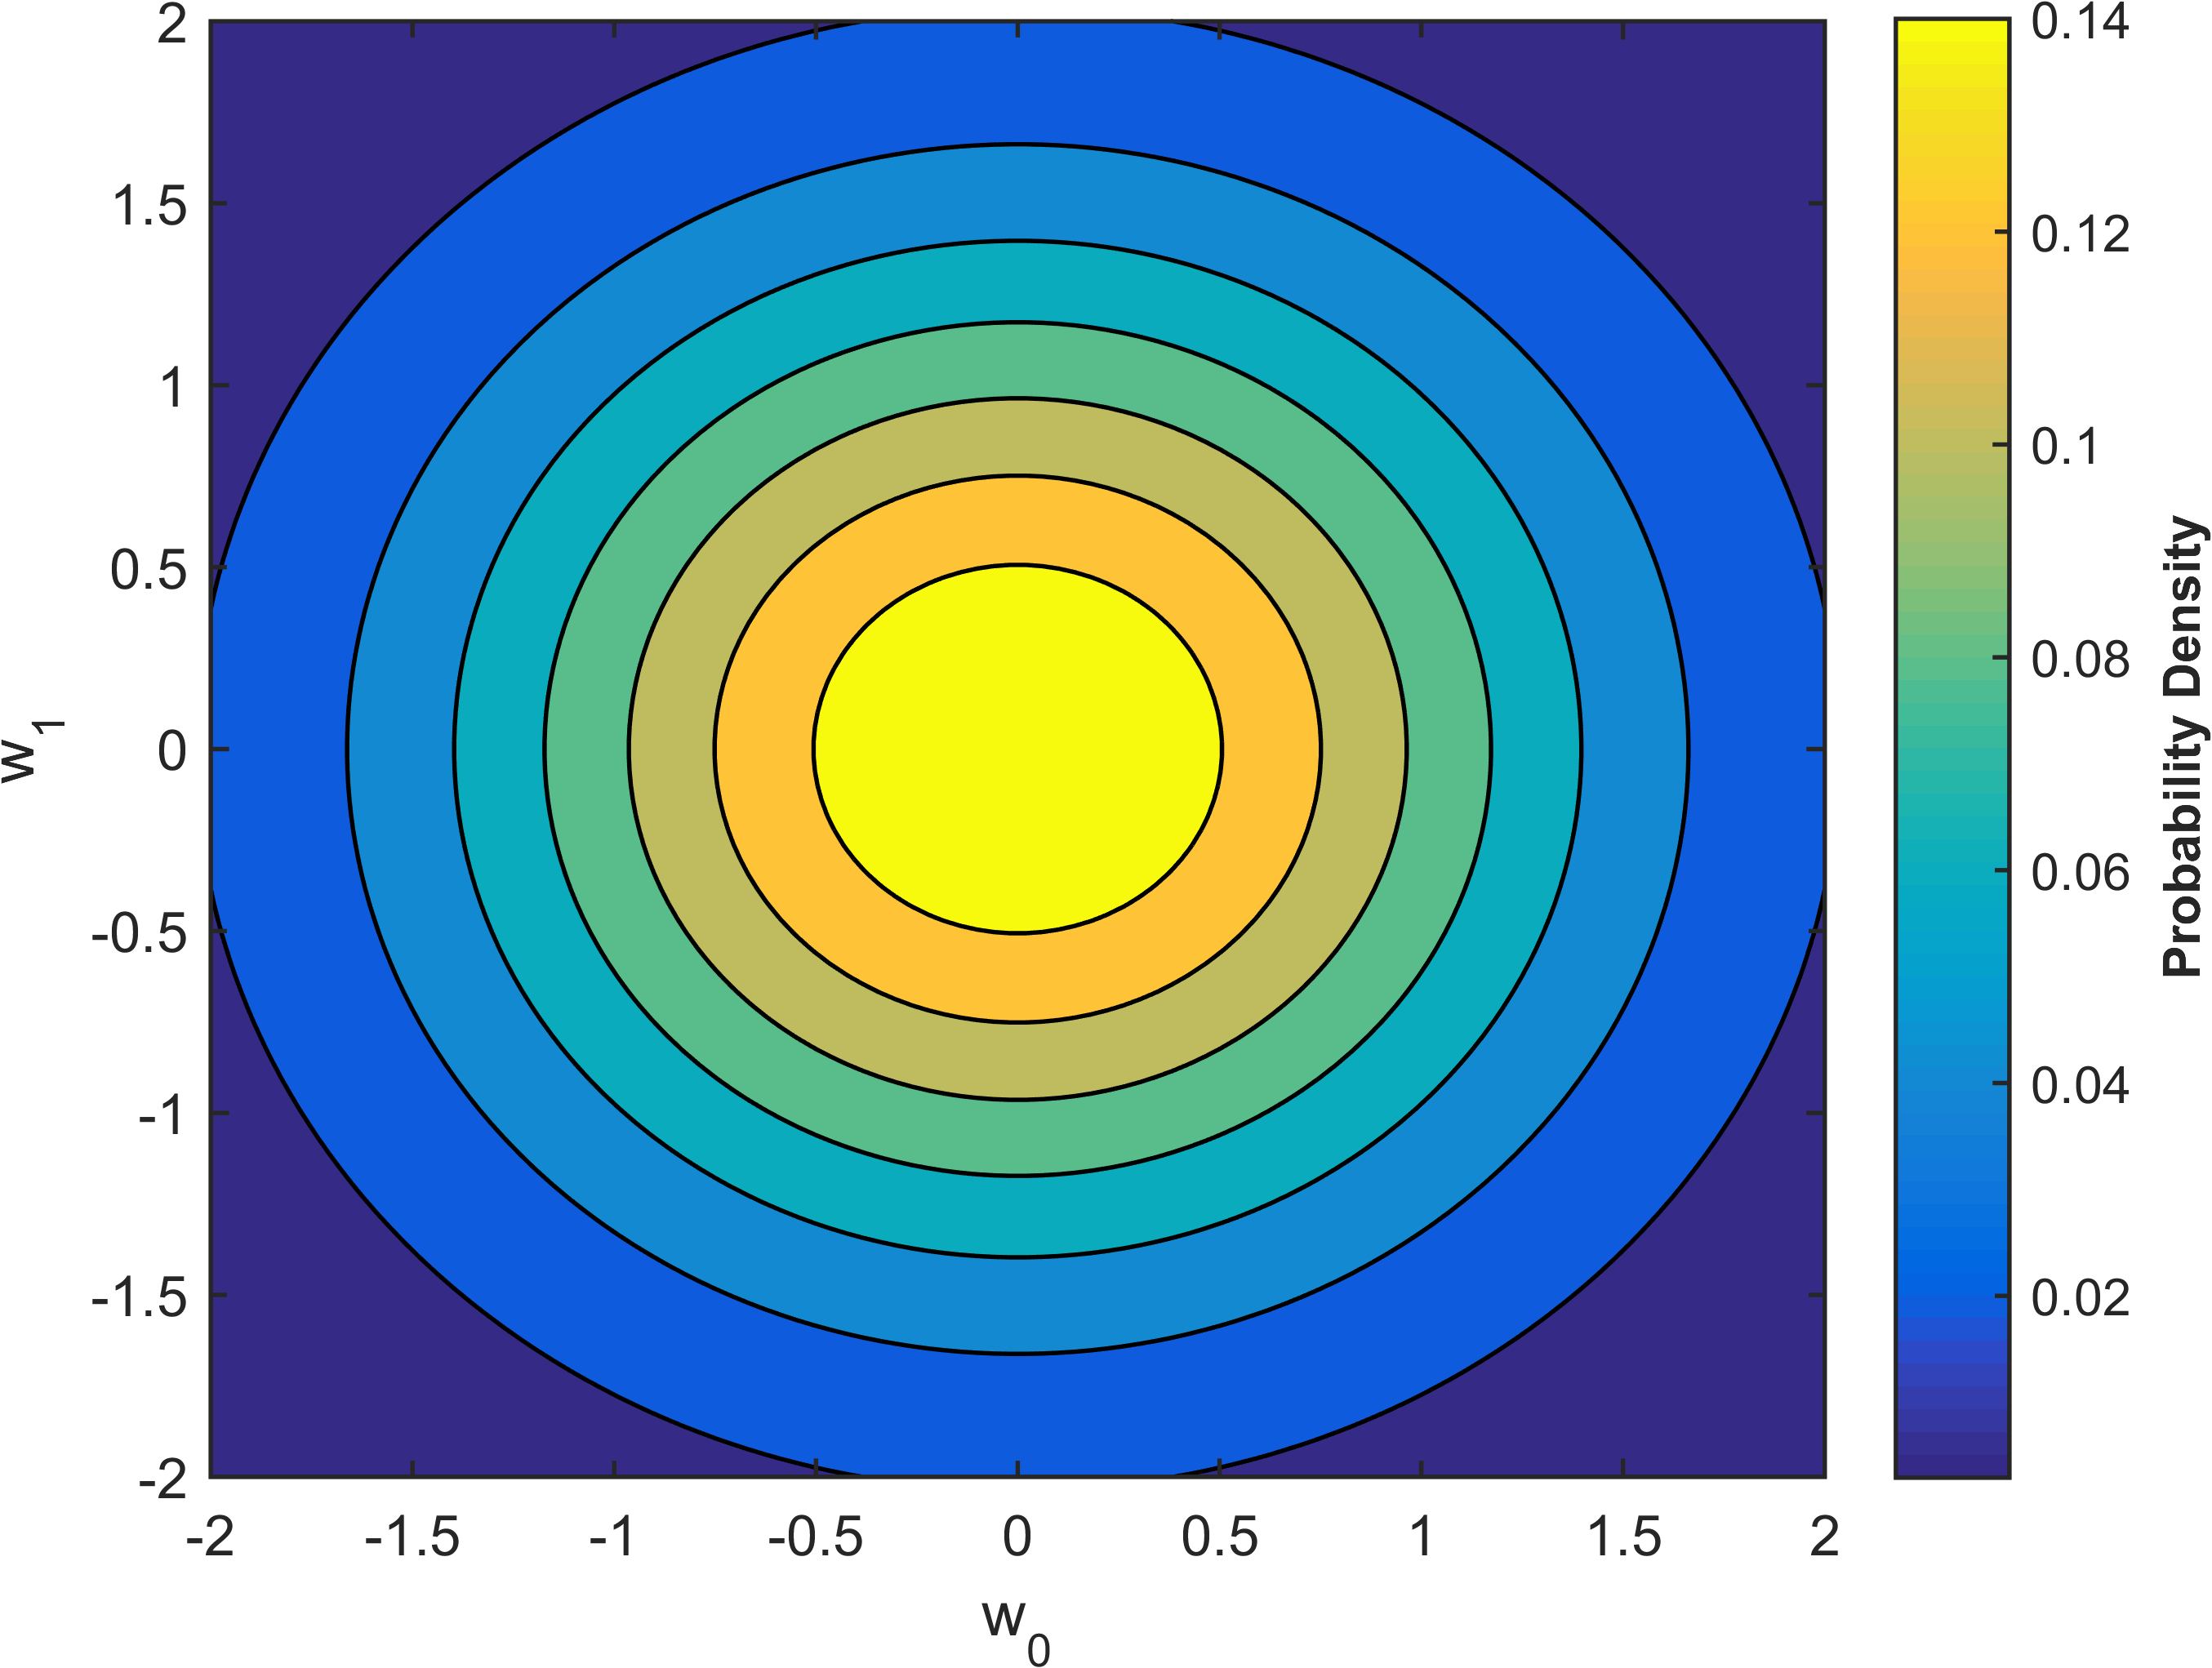
\includegraphics[width=0.45\textwidth]
        {images/part1/priorBLR}
        \label{subFigpriorBLR}
        \caption{Prior: Contours of probability density for a prior on parameters $w$ as defined by equation \ref{eqExperimentalPrior}}
\end{figure}

\begin{mdframed}[hidealllines=true,backgroundcolor=lightgray!20]
Using equations \ref{eqExperimentalPrior} and \ref{eqBayesianFunctionalPosterior} we can calculate the posterior distribution for the parameters. For a noise model of $\Pr[\epsilon] = \mathcal{N}(0, (\sigma_{n}=0.1)^2)$ the posterior distribution comes out as the figure \ref{subFigposteriorBLR}

\begin{equation}\label{eqExperimentalPosterior}
\Pr \left [\begin{pmatrix}
w_{0}\\ 
w_{1}
\end{pmatrix} \mid \mathcal{D}_{1}, \Sigma_{P}, \sigma_{n} \right ] = \mathcal{N}\left [ \begin{pmatrix}
0.2576\\ 
0.4584
\end{pmatrix}, \begin{bmatrix}
0.0037 & -0.0022\\ 
-0.0022 & 0.0138
\end{bmatrix} \right ]
\end{equation}

This simple example demonstrates how to estimate the parameters $w_{0}$ and $w_{1}$ using the prior distribution on parameters $w$ and dataset $\mathcal{D}_{1}$. The estimate of the intercept is $w_{0} = 0.2576$ and slope is $w_{1} = 0.4584$ (equation \ref{eqExperimentalPosterior}), we can use this estimate to plot the value of linear function $f(x)$ (figure \ref{subFigpredictionsBLR}). 
\end{mdframed}

\begin{figure}[!ht]
  \centering
\subfigure[{Contours of probability density for posterior distribution of parameters $w$ using equations \ref{eqExperimentalPrior} and \ref{eqBayesianPosterior}. The predicted intercept is $0.2576$ and the predicted slope is $0.4584$}]
  {
        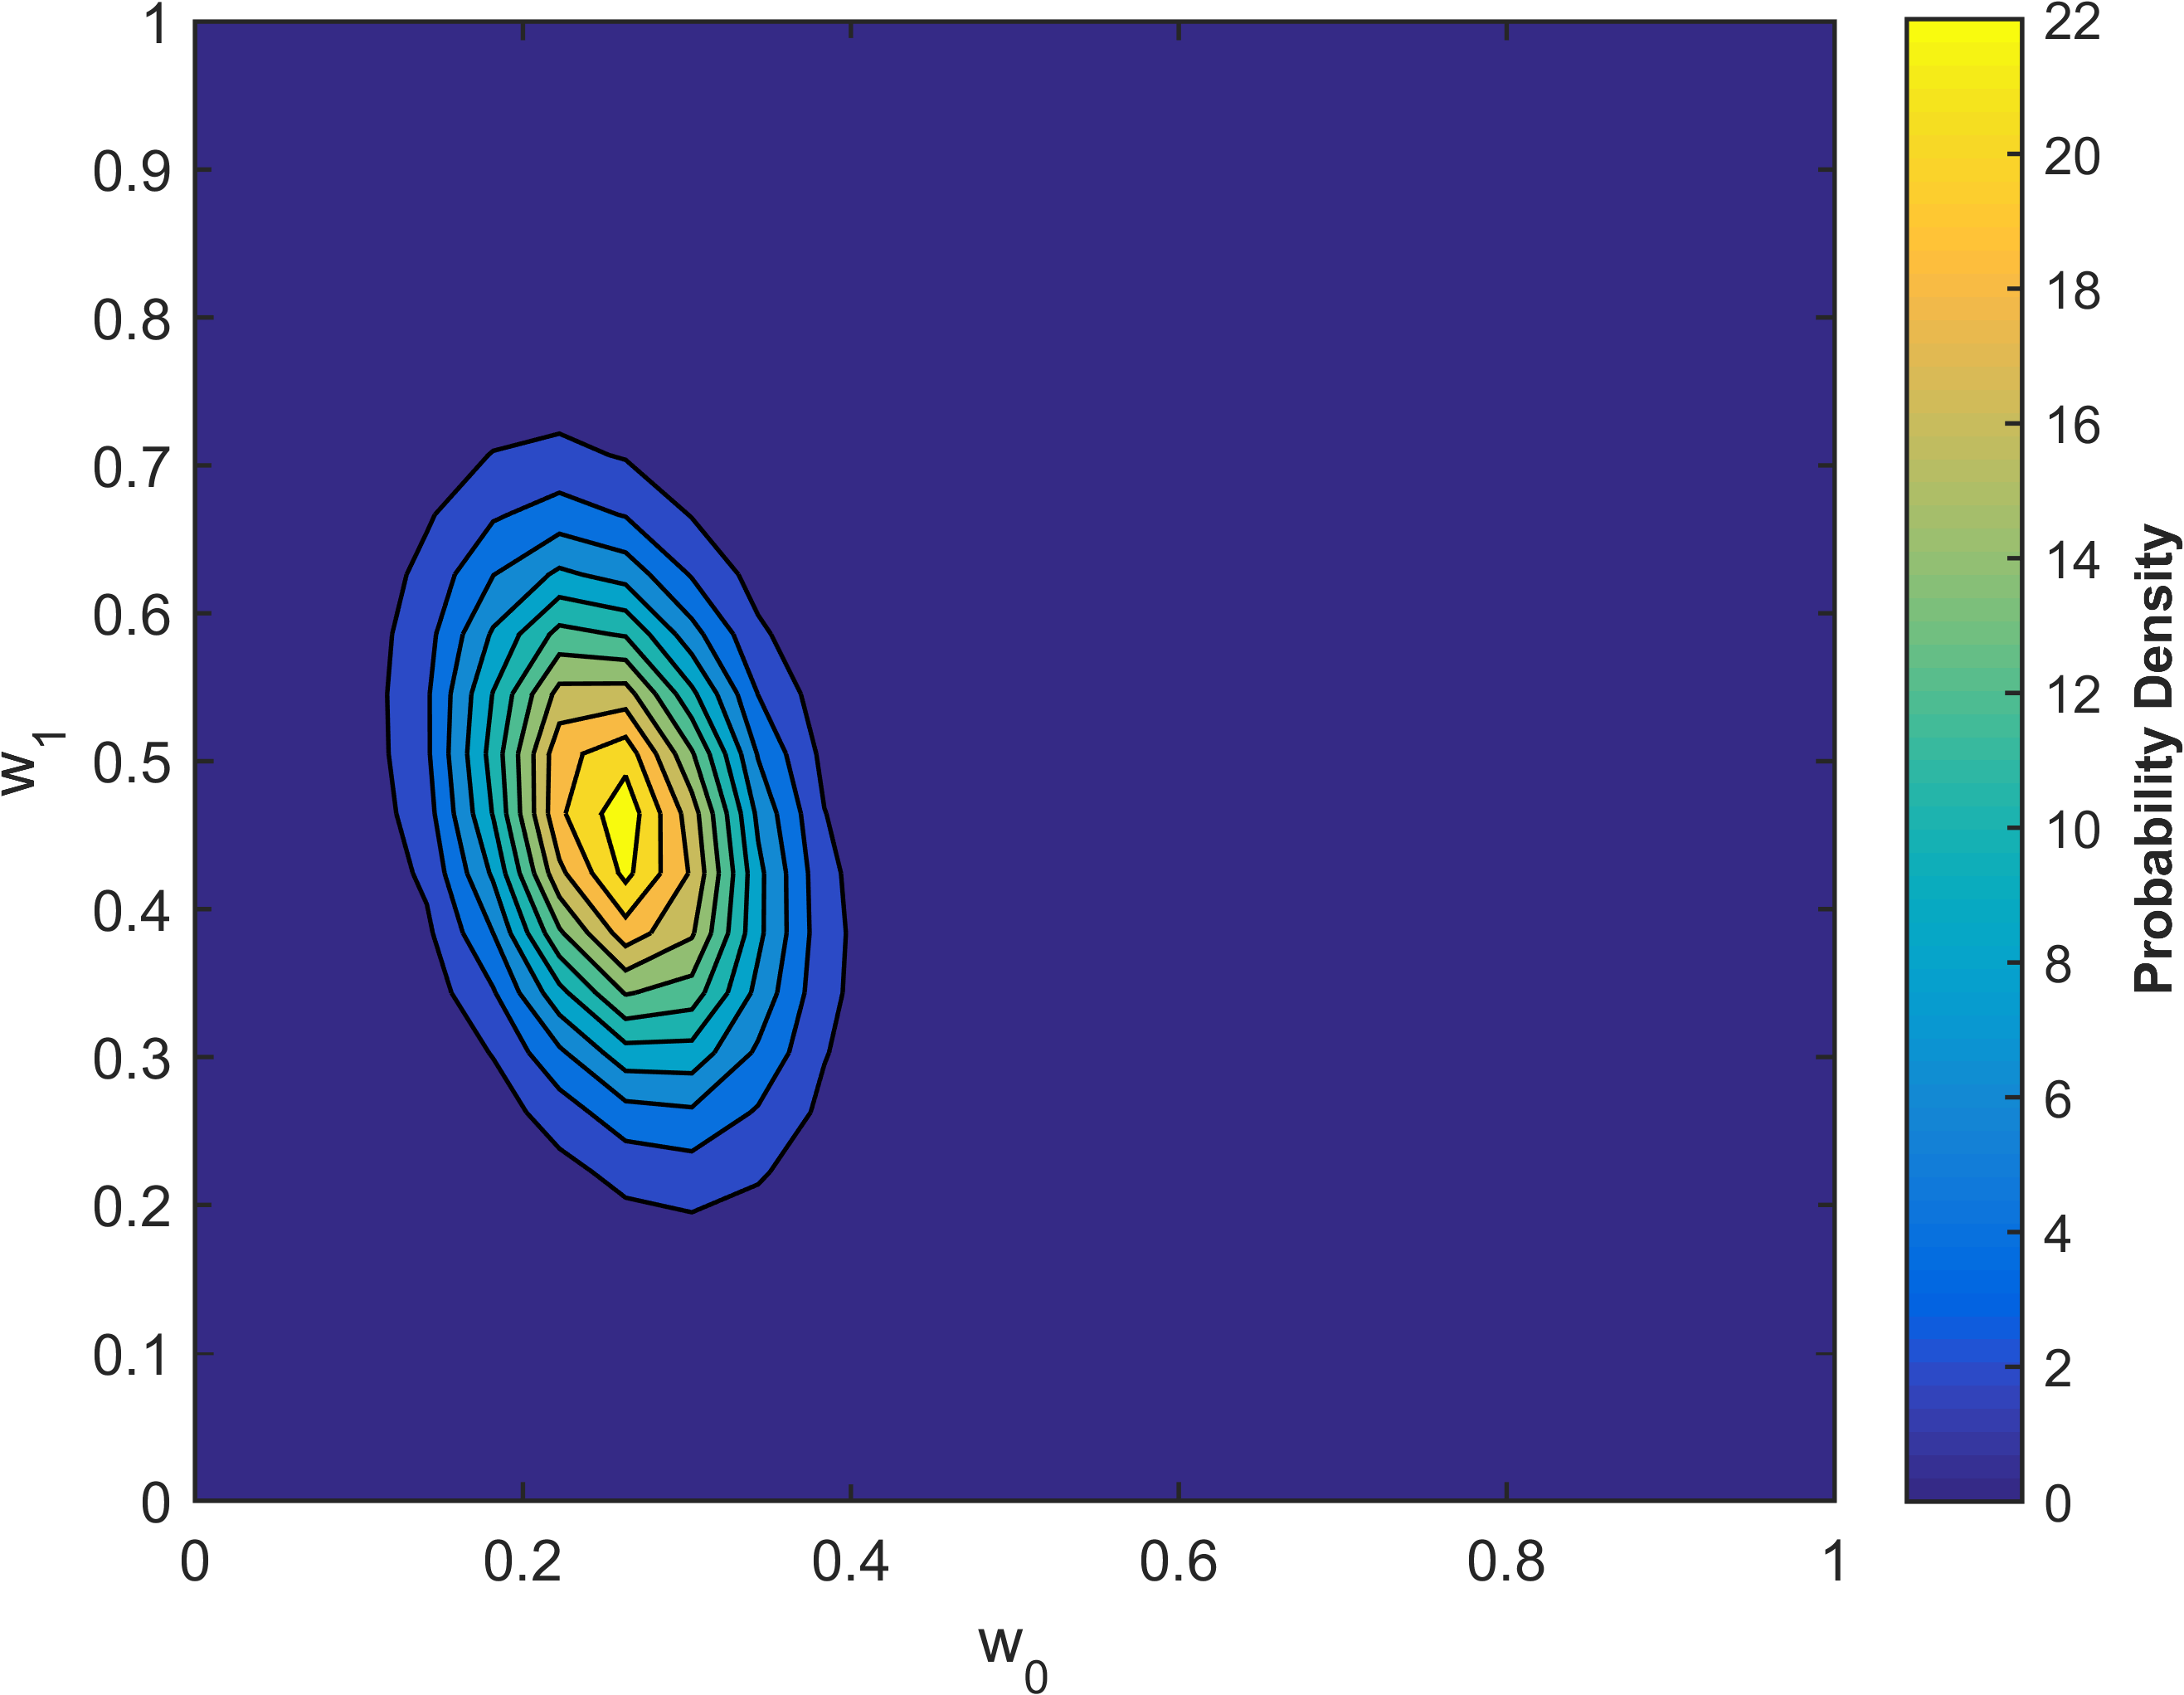
\includegraphics[width=0.45\textwidth]
        {images/part1/posteriorBLR}
        \label{subFigposteriorBLR}
  }\quad
\subfigure[{Linear Prediction based on the posterior, given the Dataset $\mathcal{D}_{1}$ prior $\Sigma_{P}$and noise $\sigma_{n}$. The predicted linear line does not pass through the data points but between them.}]
  {
        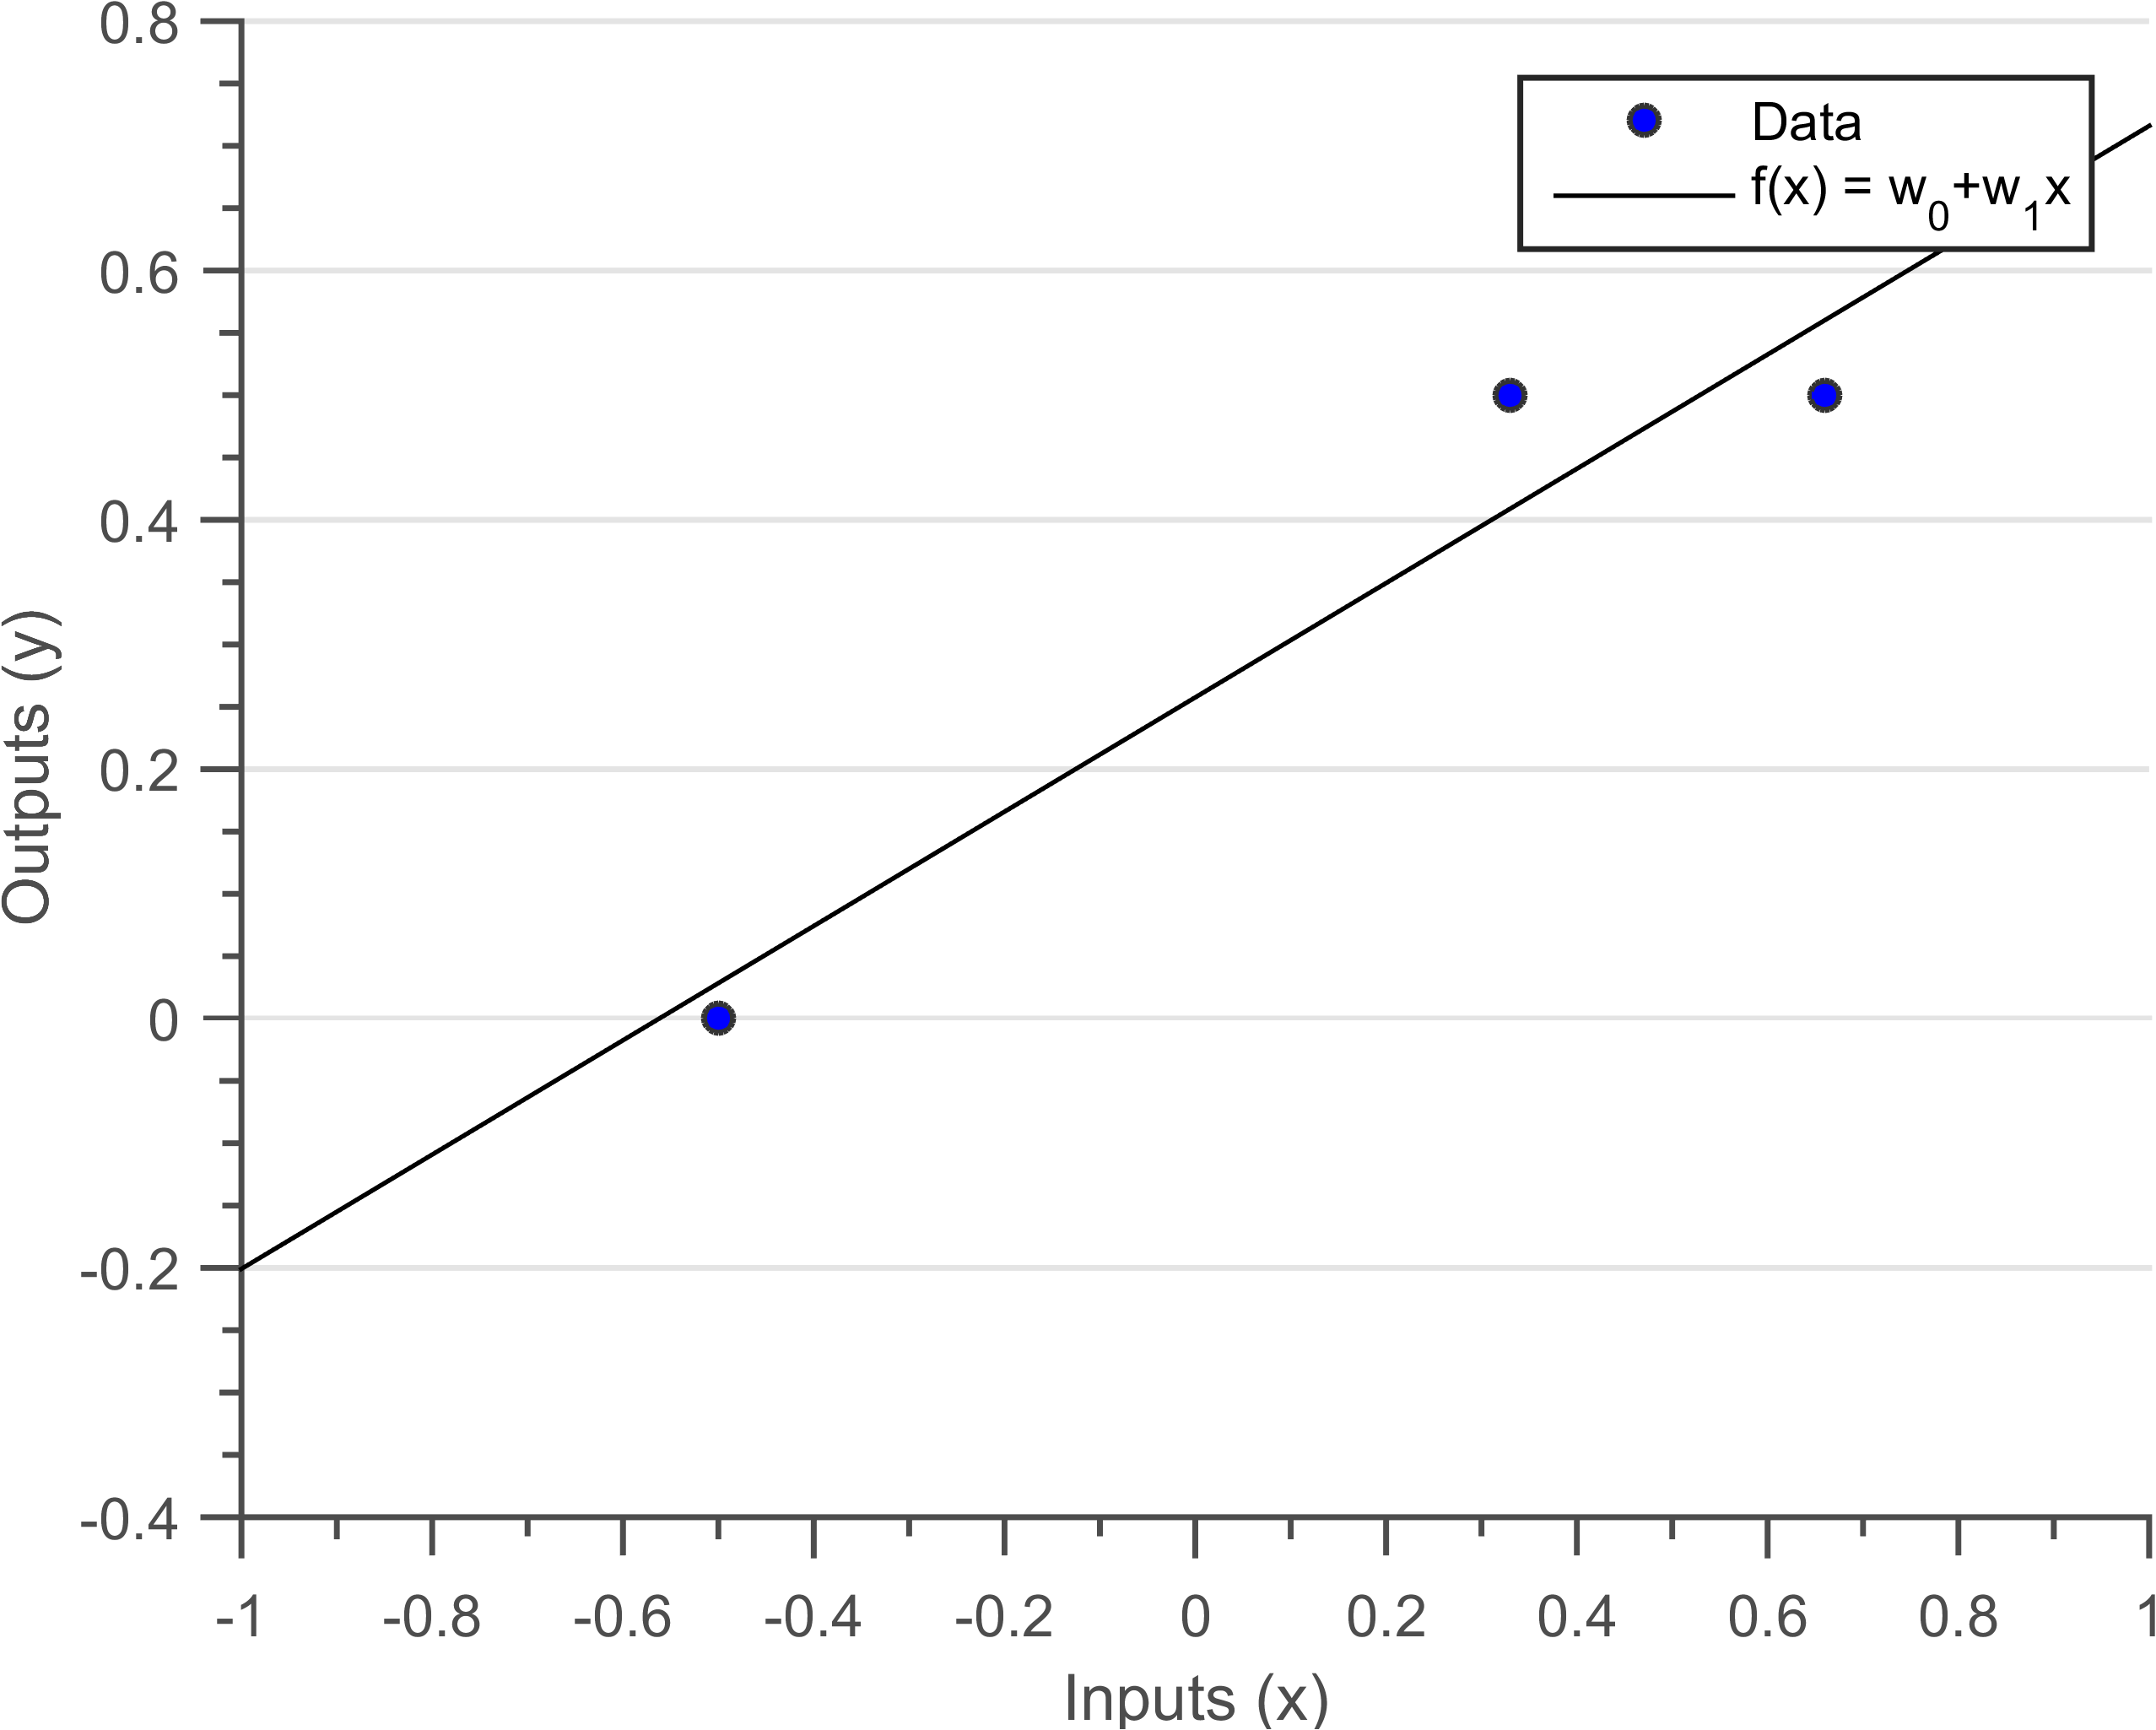
\includegraphics[width=0.45\textwidth]
        {images/part1/predictionsBLR}
        \label{subFigpredictionsBLR}
  }\quad
       \caption{Posterior and Prediction in Bayesian Linear Regression}
       \label{figPriorAndPosterior}
\end{figure}

While the Bayesian Linear Regression framework provides an opportunity to encode prior assumptions in terms of distributions of the parameters. A much more elegant and expressive method is by using GPs to perform regression. GPs are a distribution over functions and hence enable us to encode prior knowledge directly in the functional space. 

\marginnote{\textsl{Non-parametric models}}[1cm]
Learning algorithms are mainly divided into two main types. The first is defined by parametric models which can only represent a limited hypothesis space. They use parameters to describe the function between input and output domain. For example the weight parameters $w$ in Bayesian Linear Regression. The second are non-parametric models whose hypothesis space grows with the size of data \cite{ghahramani2013bayesian}. Non-parametric models use data to represent functions, GP Regression is a type of non-parametric model. One can imagine a non-parametric model like a stretched rubber sheet: whenever it sees data it deforms accordingly to compensate for the new data point. Hence the more data it sees the more it starts mimicking the actual function. 

\marginnote{\textsl{Gaussian Process}}[1cm]
Kriging was first used in the context of Geo-statistics research by Daniel Krige \cite{krige1951statistical}, this was later formalized by Matheron in his seminal work "Principals of Geo-statistics" \cite{matheron1963principles}. Recently, interest in the GPs grew in the machine learning community from neural networks research. It was shown that a Bayesian neural network becomes a GP as the number of neurons tends to infinity \cite{neal2012bayesian}. GPs are probabilistic distributions over functions, which provide a Bayesian non-parametric approach to smoothing and interpolation. Regression performed through GPs are generalizations of the Kriging algorithm. 

Informally, a GP is a method to probabilistically define a family of functions. A GP can be completely parametrized by its mean and covariance function. The mean function defines the trend-line of the family of functions, while the covariance defines the spatial dependency of input-points. Throughout this thesis we will manipulate the covariance function to encode prior known information into a GP Regression framework. 


chapter \ref{chapGp} expands GP in more detail. 

\section{Layout}\label{secOutline}
\textbf{Outine of the thesis, and on a new page}
This thesis is divided into three main parts, each part is then divided into individual chapters and their constituent sections. This part sets up the prerequisites required to understand the concepts introduced in the next two parts. The first chapter demonstrates the need for performing regression in aircraft design tasks and describes a very basic Bayesian Linear Regression scheme. 

\marginnote{\textsl{Chapter \ref{chapGp}}}[1cm]
Chapter \ref{chapGp} shows the key processes involved in a GP regression framework. GPs as distributions over functions have a rich history in geo-statistics and machine learning. The second chapter heavily draws ideas from \cite{krige1951statistical, matheron1963principles} of the geo-statistics community and \cite{Stein1999Springer, kennedy2000predicting, Rasmussen2005, mackay2003information} of the machine-learning community, showing a process flow of how to perform regression using GPs. The remaining chapter unfolds as follows, section \ref{secPrior} describes the key constituents of a GP and how to draw random functions from a GP. Section \ref{secPosterior} describes how to perform prediction in presence and absence of measurement noise. Section \ref{secHyperParameter} introduces marginal likelihood as a form of evaluation method to automatically choose hyper-parameters. 

\marginnote{\textsl{Chapter \ref{chapScalingGPR}}}[1cm]
Chapter \ref{chapScalingGPR} deals with the problem of scaling GP regression to massively many points. Traditional GPs are computationally infeasible on a standard laptop if the number of data points increase $\mathcal{O}(10^4)$. There exist two main methods to scale a GP regression, one using reduced set of inducing points while another based on mixture of experts methodology. This chapter draws heavily from the works of \cite{quinonero2005unifying, seeger2003fast, Snelson06sparsegaussian, Titsias09variationallearning} for the approximation method of inducing points and \cite{cao2014generalized, tresp2000bayesian, chen2009bagging, deisenroth2015distributed} for the approximation method of mixture of experts, please refer to the individual publications for more detail. We demonstrate the limitations and capabilities of both the methods on a toy dataset, giving directions to choosing optimal parameters and extracting the best possible result.  

\textbf{Description of the other two parts}

\textbf{Contributions}

%%% Local Variables: 
%%% mode: latex
%%% TeX-master: "isae-report-template"
%%% End: 
